\documentclass{report}
\usepackage{graphicx}
\graphicspath{ {./images/} }
%%%%%%%%%%%%%%%%%%%%%%%%%% Practice info %%%%%%%%%%%%%%%%%%%%%%%%%%
\Subject {Системи штучного інтелекту}
\LabTitle{Логістична регресія}
\LabReport{Практична робота \#3}

\Done{Виконав:}  % Поставте правильне закінчення

%%%%%%%%%%%%%%%%%%%%%%%%%% Your personal data %%%%%%%%%%%%%%%%%%%%%%%%%%
\Surname{Коваль}
\Name{Ростислав}
\Group {ІО-11мн}
\YearOfStudying {1}

%%%%%%%%%%%%%%%%%%%%%%%%%% starting the document %%%%%%%%%%%%%%%%%%%%%%%%
\startDocument


\section{Логістична регресія}

\subsection{Письмове завдання}

Покажіть, що похідна сигмоїди дорівнює цьому виразу:

\begin{equation}
  \begin{split}\tikzmarkin[fill=lightgray]{y}(0.2, -0.5)(-0.2, 0.65)
  \frac{d \hat y}{dx} = \frac{d \sigma(z)}{dx} = \sigma(x)\big (1 - \sigma(x) \big ),
  \tikzmarkend{y}
  \end{split}
\end{equation}


де $ \hat y = \sigma(x) = \frac{1}{1 + \exp{(-x)}}$

\vspace{0.5cm}
\textbf{Розв'язок:} % Розмістіть нижче свій розв'язок

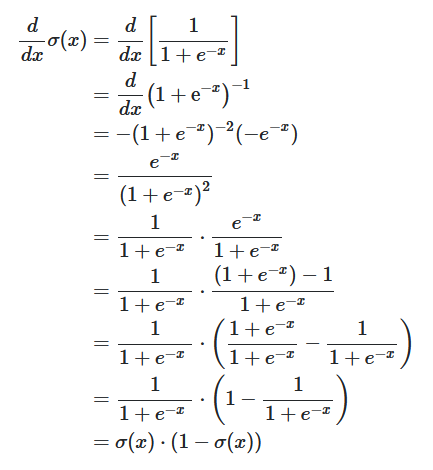
\includegraphics{images/deriv.png}


\subsection{Завдання з програмування}

\begin{lstlisting}[language=Python, style=mypython, caption={Ініціалізація вагів та зсуву}]
def parameters_inititalization():
  W = np.zeros((50310, 1))
  b = 0
  return W, b
\end{lstlisting}
\begin{lstlisting}[language=Python, style=mypython, caption={Застосування нелінійної функції активації (сигмоїди) до лінійної комбінації вхідних ознак та ваг, включаючи зсув}]
def forwardPropagate(X, W, b):
z = np.dot(W.T, X) + b
y_hat = 1 / (1 + np.exp(-z))
return z, y_hat
\end{lstlisting}
\newpage
\begin{lstlisting}[language=Python, style=mypython, caption={Обчислення усередненої втрати на всьому навчальному наборі даних. Цільова функція}]
def cost(n, y_hat, y_true):
mult = np.multiply(y_true, np.log(y_hat)) + np.multiply((1 - y_true), np.log(1 - y_hat))
J = - np.sum(mult) / n
return J
\end{lstlisting}
\begin{lstlisting}[language=Python, style=mypython, caption={Розрахунок градієнтів цільвої функції відносно ваг та зсуву}]
def backwardPropagate(n, X, y_hat, y_true):
dW = np.dot(X, (y_hat - y_true).T) / n
db = np.sum((y_hat - y_true)) / n
return dW, dbE
\end{lstlisting}
\begin{lstlisting}[language=Python, style=mypython, caption={Оновлення вагів та зсувів}]
def update(alpha, dW, db, W, b):
W = W - alpha * dW
b = b - alpha * db
return W, b
\end{lstlisting}
\begin{lstlisting}[language=Python, style=mypython, caption={Тестування}]
def testing():
W, b = parameters_inititalization()
for i in range(100):
z, y_hat = forwardPropagate(norm, W, b)
J = cost(1, y_hat, y_true)
dW, db = backwardPropagate(1, norm, y_hat, y_true)
W, b = update(0.003, dW, db, W, b)
print(J)
testing()
\end{lstlisting}


\subsection{Результати експериментів}
Деталі дослідження представлені у вигляді таблиць.
Для alpha = 0.0001:


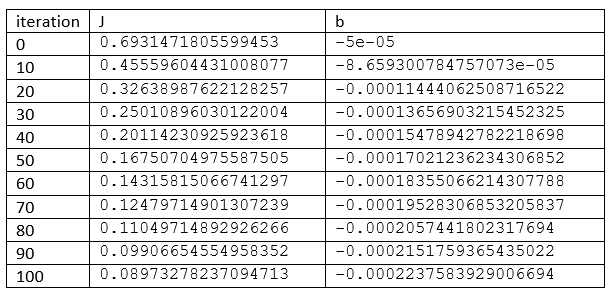
\includegraphics{images/00001.png}
\newpage
Для alpha = 0.003:

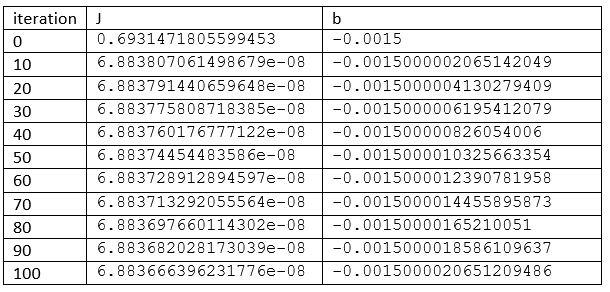
\includegraphics{images/0003.png}

З таблиці можна зробити висновок, що при більшій швидкості навчання значення цільової функції з кожною ітерацією стає значно меншим, що свідчить про здійснення навчання. Значення зсуву є більшим при alphа = 0.003. Значення вагів представляються у вигляді великого масиву, тому недоречно вставляти його в таблицю порівняння. Їх значення змінюються при кожній ітерації.

\subsection{Допомога}
Не отримував допомоги від інших людей, використовував наступні матеріали:
~\cite{overleaf, git1, git2, calculus}.

\subsection{Висновки}
Упродовж виконання лабораторної роботи було спостережно, що значення цільової функції зменшується при кожній ітерації, при збільшенні швидкості навчання значення функції значно зменшується. Значення зсуву моделі незначно зменшується, можна вважати, значення вагів також змінюється.

\newpage
%%%%%%%%%%%%%%%%%% Література %%%%%%%%%%%%%%%%%%%%%%%%%%%%%%%%%%%%%%%%%%%%%%%
\clearpage
\bibliographystyle{IEEEtran}
\bibliography{ref}
\end{document}
